\documentclass[11pt,conference,draftcls,onecolumn]{IEEEtran}
\pagestyle{plain}
\IEEEoverridecommandlockouts
% The preceding line is only needed to identify funding in the first footnote. If that is unneeded, please comment it out.
\usepackage{cite}
\usepackage{amsmath,amssymb,amsfonts}
\usepackage{algorithmic}
\usepackage{graphicx}
\usepackage{textcomp}
\usepackage{xcolor}
\usepackage{listings}
\def\BibTeX{{\rm B\kern-.05em{\sc i\kern-.025em b}\kern-.08em
    T\kern-.1667em\lower.7ex\hbox{E}\kern-.125emX}}
\begin{document}

\title{Online Anomaly Detection in Request-Based Battery Management Systems\\
{}
\thanks{This work was funded in part by NSF Grant No. 1234567}
}

\author{\IEEEauthorblockN{Aaron Willcock}
\IEEEauthorblockA{\textit{Department of Computer Science} \\
\textit{Wayne State University}\\
Detroit, MI, USA \\
aaron.willcock@wayne.edu}
\and
\IEEEauthorblockN{Nathan Fisher}
\IEEEauthorblockA{\textit{Department of Computer Science} \\
\textit{Wayne State University}\\
Detroit, MI, USA \\
fishern@wayne.edu}
}

\maketitle

\begin{abstract}
Battery Management System (BMS) research has included reconfigurable cell architecture, state of health estimation, battery balancing, and real-time scheduling.
However, anomaly detection in BMSs is addressed only as an offline method for identifying malfunctions or parasitic loads.
Furthermore, the costly implementation of BMSs has resulted in few works evaluating approaches outside of simulation.
In this report, a low-cost BMS is designed and implemented with an online anomaly detection system to mitigate damage in real-time.   
\end{abstract}

\begin{IEEEkeywords}
battery management system, anomaly detection, real-time systems
\end{IEEEkeywords}

\section{Introduction}
The number of plug-in electric vehicles (hybrid and pure-electric) is expected to reach over 70 million by 2030 according to the International Energy Agency \cite{iea}.
Electric vehicles typically contain a Battery Management System (BMS) responsible for handling the charging, discharging, reconfiguration, monitoring and control of the vehicles batteries.
Recent BMS research has included architecture of reconfigurable cells, state of health estimation, battery balancing, and real-time scheduling
\cite{batteryAwareDynamicSchedulingForPeriodicTaskGraphs,realTimePredictionOfBatteryPowerRequirements,reconfigurableBatteryTechniquesAndSystems}.
However, BMSs are expensive to purchase and as a result many research projects concerning BMS architecture (both physical and digital) are evaluated in simulation only \cite{towardsSmarterBatteryDesign}.
To the best of our knowledge, few works have implemented a low-cost BMS system and no works have addressed online anomaly detection in the operation and communication of BMSs.
Furthermore, we are not aware of any works which govern BMS supply on a request basis.

As such, we view the lack of online anomaly detection in BMS operation and communication as an opportunity to design fault-detection behavior for load-aware BMS.
The absence of request-based in existing BMS architectures is another opportunity for applying real-time systems concepts to anomaly detection.
Finally, this project tangentially addresses the challenge of producing a low-cost physical realization to help make BMS implementation and testing more accessible by lowering the cost of entry.

\subsection{Research Questions and Project Goal}
Formally, our research questions are as follows:
\begin{enumerate}
    \item What anomalies can exist in a BMS?
    \item How can request-based communication between a load manager and BMS be used to implement and/or improve anomaly detection?
    \item What design would facilitate a low-cost implementation and evaluation of online anomaly detection in a request-based BMS?
\end{enumerate}

The overarching goal of this project is to create a joint Load Management System (LMS) and BMS that is: low cost in manufacturing and materials cost;
allows for the creation, acceptance, rejection, and enforcement of load schedules;
and detects system anomalies including over-voltage, under-voltage, over-current, under-current, and load mismatch.

\subsection{Contributions}
The contributions of this project report are summarized as:
\begin{enumerate}
    \item a low-cst BMS-LMS model,
    \item a protocol for request-based BMS-LMS communication,
    \item a set of online anomaly detection methods based on the above model and protocol, and
    \item a low-cost BMS-LMS system implementation that demonstrates anomaly detection.
\end{enumerate}

Additionally, this report along with all source code can be found on GitHub at:
https://github.com/
aarontwillcock/ece5280cps-ubms

\subsection{Report Outline}
The remainder of the report is as follows.
Section \ref{sec:relatedWork}, Related Work, covers related work in topics including batteries, battery management systems, and real-time systems.
Section \ref{sec:systemModel}, System Model, defines the system model including the Battery Management and Load Management Systems.
Section \ref{sec:rbComm}, Request-Based Communication, explains the request-based communication protocol.
Section \ref{sec:anomalyDetection}, Anomaly Detection, discusses the types of anomalies that may occur in BMSs and the approaches taken to detect them in this project.
Section \ref{sec:experiments}, Experiments, lists the experimental setup, execution, and experiments themselves to evaluate the efficacy of the online anomaly detection approach.
Section \ref{sec:results}, Results, describes the results of the aforementioned experiments.
Section \ref{sec:discussion}, Discussion, identifies weaknesses in the model and approach, implementation challenges, and deferred objectives.
Section \ref{sec:conclusion}, Conclusion, concludes the report with a summary of contributions and future work. 

\section{Related Work}\label{sec:relatedWork}
The state-of-the-art in battery management systems as it pertains to real-time systems focuses on two topics: batteries (and the BMSs that manage them) and real-time, cyber-physical systems.
Work that focus on batteries or BMSs exclusively tend to be hardware-oriented while cyber-physical and real-time systems works are either a blend of hardware and algorithms or algorithms exclusively.
The following subsections highlight some relevant works in these topics.

\subsection{Batteries and Battery Management Systems}
Relevant battery-specific research includes recent works on software-defined batteries \cite{softwareDefinedBatteriesConf,softwareDefinedBatteriesJrnl}.
In software-defined batteries, batteries of different chemistries may be combined to leverage the benefits of both chemistries.
Through fast switching, battery charging and discharging can be optimized by distributing the energy load according to battery type.

In a less-flexible sense, other batteries leverage software to closely monitor individual cells and provide load balancing across those cells with the goal of extending battery lifetime \cite{towardsSmarterBatteryDesign}.

Other works address the design of switches around batteries to maximize reconfigurability of batteries while minimizing hardware cost \cite{reconfigurableBatteryTechniquesAndSystems}.
In reconfigurable batteries, cells may rearrange the order in which electrons pass through them (ex. series vs parallel) to change maximum current and voltage delivery online.
Reconfigurable batteries also allow the BMS to completely remove cells which are reducing the performance of neighboring cells \cite{aCaseStudyOnImprovingCapacityDeliveryOfBatteryPacksViaReconfiguration}.

\subsection{Real-Time and Cyber-Physical Systems}
From the cyber-physical and real-time systems perspective, research on BMSs may be aware of electro-chemical properties and hardware cost but focuses more on exploitable properties of the hardware, computational cost, and scheduling.

In the most inflexible case of battery management systems, Liang He provided an approach for state of health estimation in mobile devices which lack coulomb counters \cite{batterySoHEstimationMobile}.
Other works address real-time prediction of power requirements for hybrid and electric vehicles \cite{realTimePredictionOfBatteryPowerRequirements} and online thermal management for BMSs \cite{realTimeBatteryThermalManagement}.

From a pure scheduling standpoint, some works provide scheduling approaches that leverage Dynamic Voltage and Frequency Scaling (DVFS) along with models of constrained power supplies (batteries) to maximize computation while minimizing energy usage (thus extending the amount of computation which may be performed) \cite{batteryAwareDynamicSchedulingForPeriodicTaskGraphs}.

\section{System Model}\label{sec:systemModel}

Motivated by the absence of online anomaly detection for battery management systems, the following section provides an overview of the system model and its two primary components: the BMS and the Load Management System (LMS).

\subsection{System Overview}
The proposed system model contains both a BMS and LMS which act as two nodes in control of the supply and demand of energy respectively.
Figure \ref{fig:bmsModel} depicts a high-level schematic of what devices the BMS and LMS are connected to and responsible for.
The BMS is responsible for monitoring current flow out of the cell.
The LMS is responsible for characterizing the attached system loads and communicating with the BMS over UDP to request permission to active the system loads.
The following subsections will describe implementation-specific points about the BMS and LMS.
\begin{figure}[!htbp]
    \centering
    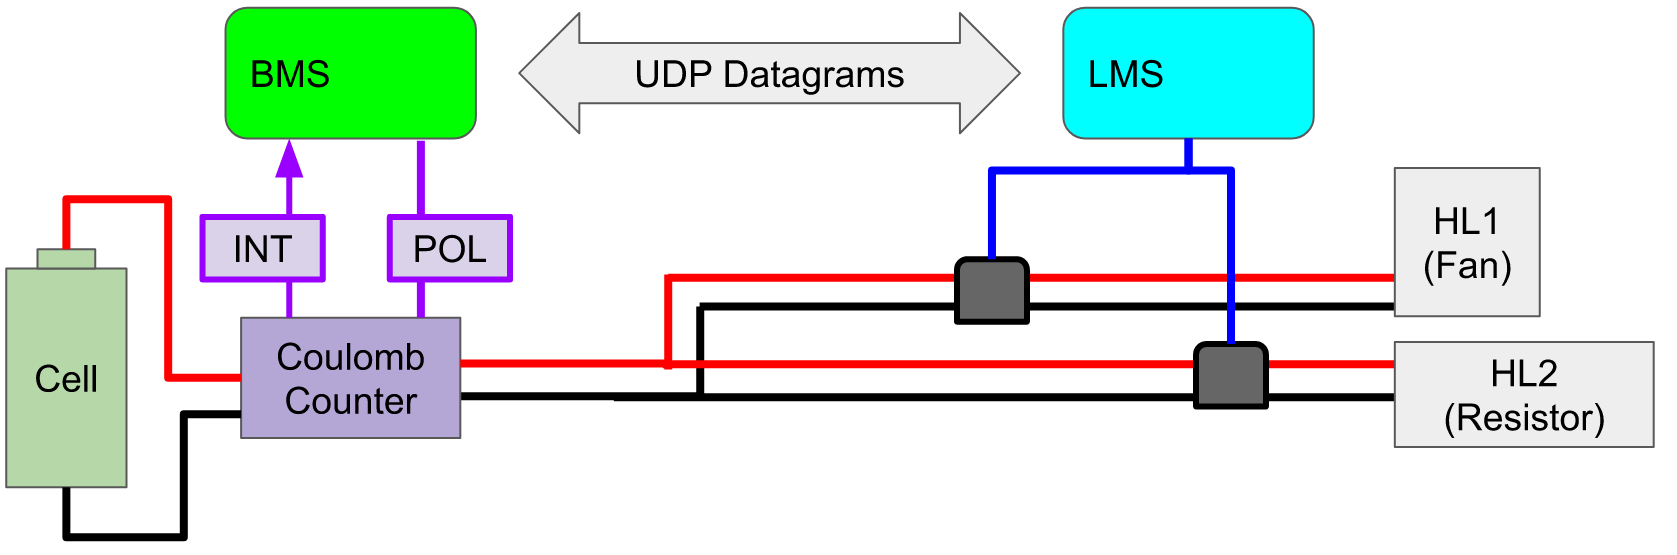
\includegraphics[width=6.5in]{img/uBmsModel.png}
    \caption{BMS and LMS Schematic}
    \label{fig:bmsModel}
\end{figure}
\clearpage
\subsection{Battery Management System Architecture}
In the implementation, the BMS is a Raspberry Pi Zero W \cite{rpiZeroW} which is connected to an LTC4150 Coulomb Counter breakout board.
Figure \ref{fig:coulombCounter} depicts the LTC4150 Coulomb Counter breakout board and its pin names.
The LTC4150 Coulomb Counter breakout board is connected to the nickel–metal hydride (NiMH) battery cells pictured in Figure \ref{fig:nimhBatt}.
Each NiMH cell provides 1.2 V and around 1200mAh of charge.
The NiMH configuration for this project was four cells in series bringing the voltage to 4.8V while maintaining 1200mAh of charge.
This battery model is stored in the BMS for use in accepting and rejecting loads that match the battery configuration - as will be discussed later.

The Raspberry Pi Zero W is configured to fire an interrupt service routine (ISR) on each falling edge of the General Purpose Input-Output (GPIO) port connected to the interrupt port (INT) of the LTC4150 Coulomb Counter (see figure for INT pin).
The LTC4150 Coulomb Counter's INT pin voltage falls low (signaling an interrupt) each time 0.614439C flows through the IN pins and out through the OUT pins - in either direction.
The polarity pin (POL) indicates the in which the 0.614439C has traveled.
By sampling the POL pin each time the ISR is fired, the BMS may track the current flow through (and remaining charge in) the monitored battery. 

The BMS, being a Raspberry Pi Zero W, is also equipped with a wireless interface which is used to communicate with the LMS over UDP.
\begin{figure}[!htbp]
    \centering
    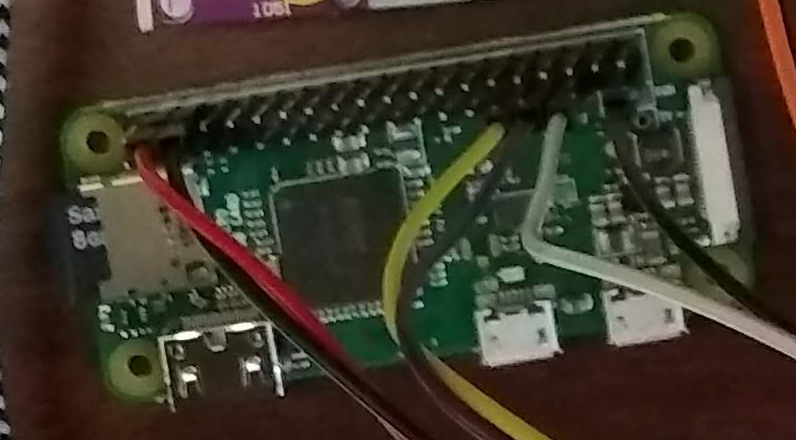
\includegraphics[width=3.5in]{img/rpi0w.png}
    \caption{Raspberry Pi Zero W as a BMS}
    \label{fig:rpi0w}
\end{figure}
\begin{figure}[!htbp]
    \centering
    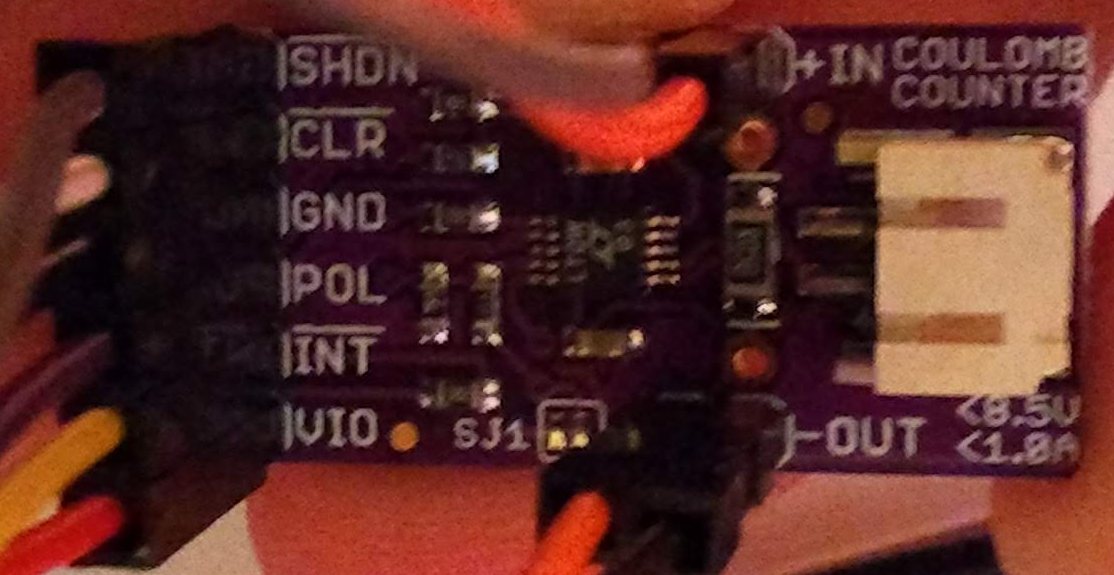
\includegraphics[width=4.5in]{img/coulombCounter.png}
    \caption{An LTC4150 Coulomb Counter Breakout Board}
    \label{fig:coulombCounter}
\end{figure}
\begin{figure}[!htbp]
    \centering
    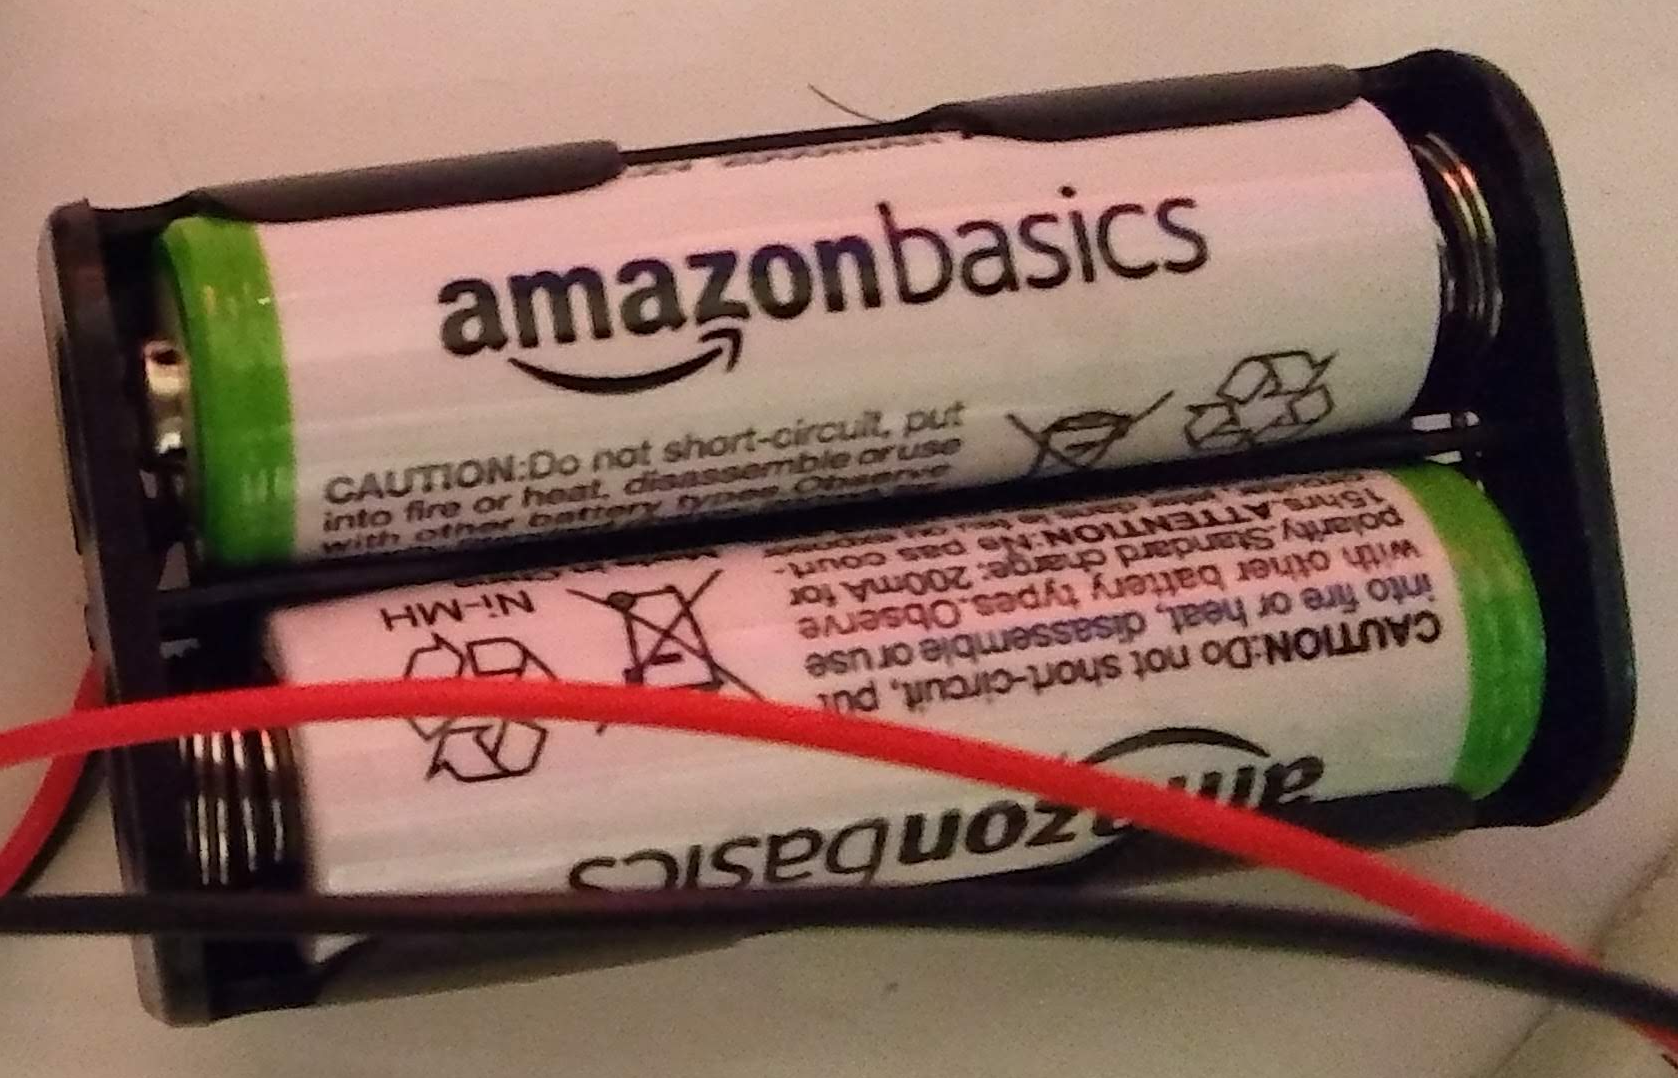
\includegraphics[width=3.5in]{img/nimhBatt.png}
    \caption{1.2V Ni-Mh Batteries}
    \label{fig:nimhBatt}
\end{figure}

\subsection{Load Management System Architecture}
The LMS is a Raspberry Pi 3 which is connected to two PN2222a transistors \cite{pn2222a}.
The first PN2222a transistor, when active, connects the NiMH-supplied power to the 6V 130-size DC motor \cite{130motor}.
The second PN222a transistor, when active, connects the NiMH-supplied power to a 100 Ohm resistor.

The LMS maintains a model of each load and uses these models to request power be supplied by the BMS as will be described later.
The LMS performs all requests over UDP via the built-in Raspberry Pi 3 wireless interface.
Figure \ref{fig:rpi3} shows the Raspberry Pi 3 (LMS), several PN2222a transistors used to activate and deactivate loads, the fan, and several resistors used as loads. The additional resistors and transistors not described here are covered in the Deferred Objectives subsection of Section \ref{sec:discussion}, Discussion.
\begin{figure}[!htbp]
    \centering
    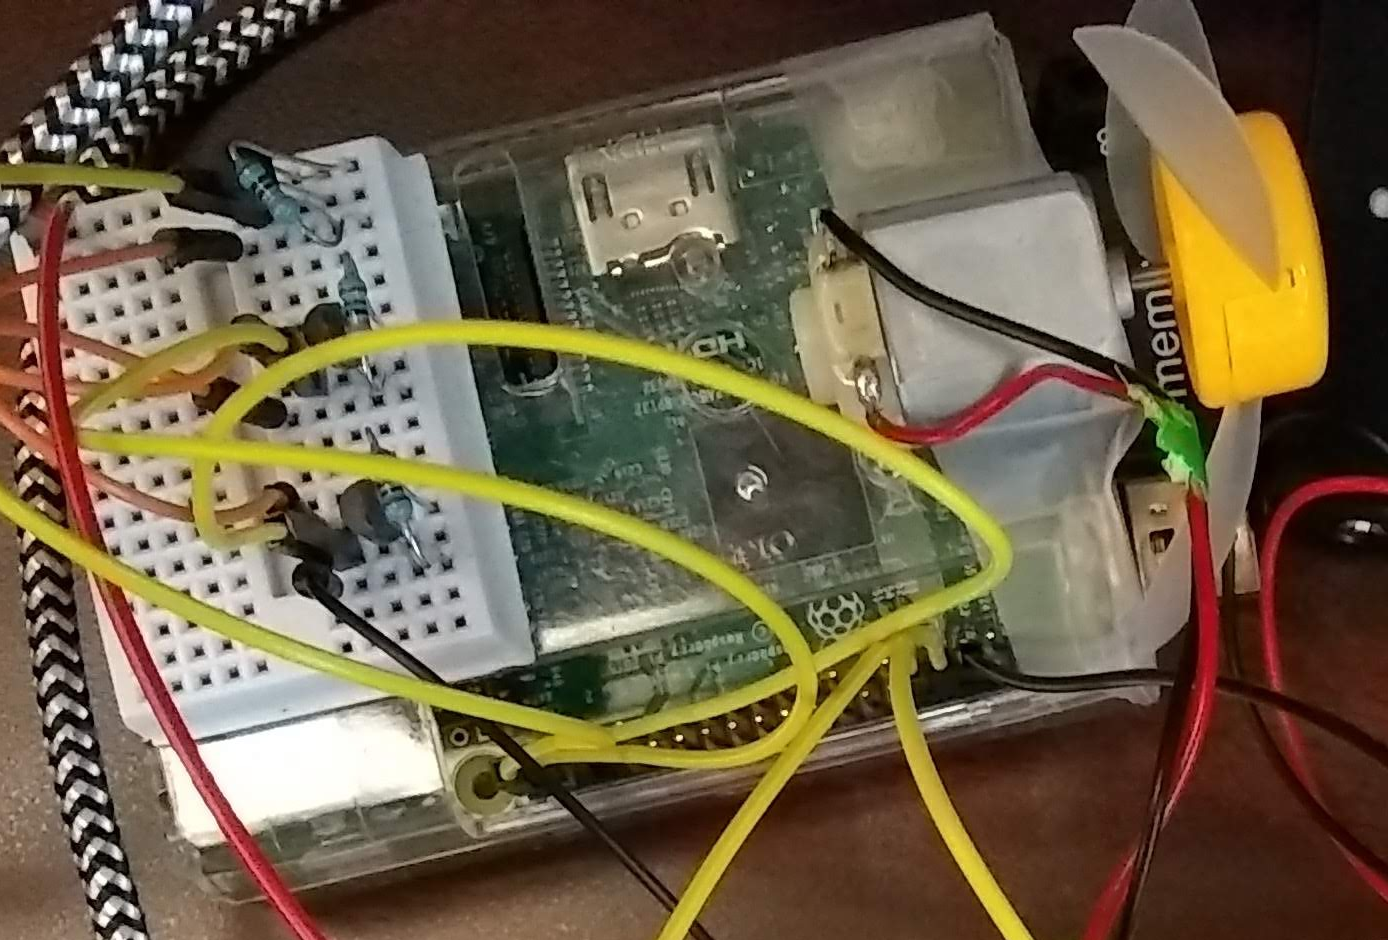
\includegraphics[width=6.5in]{img/rpi3.png}
    \caption{Raspberry Pi 3}
    \label{fig:rpi3}
\end{figure}

\subsection{System Model Summary}
To place all hardware in perspective, Figure \ref{fig:bmsModelPics} shows the photos of each system atop the high-level schematic.
An important difference in the implementation from the schematic presented is that both Raspberry Pis (the BMS and LMS) are powered via their USB power inputs as each Raspberry Pi contains protection circuitry.
Thus, the only loads powered by the NiMH batteries are the fan and 100 Ohm resistor.
\begin{figure}
    \centering
    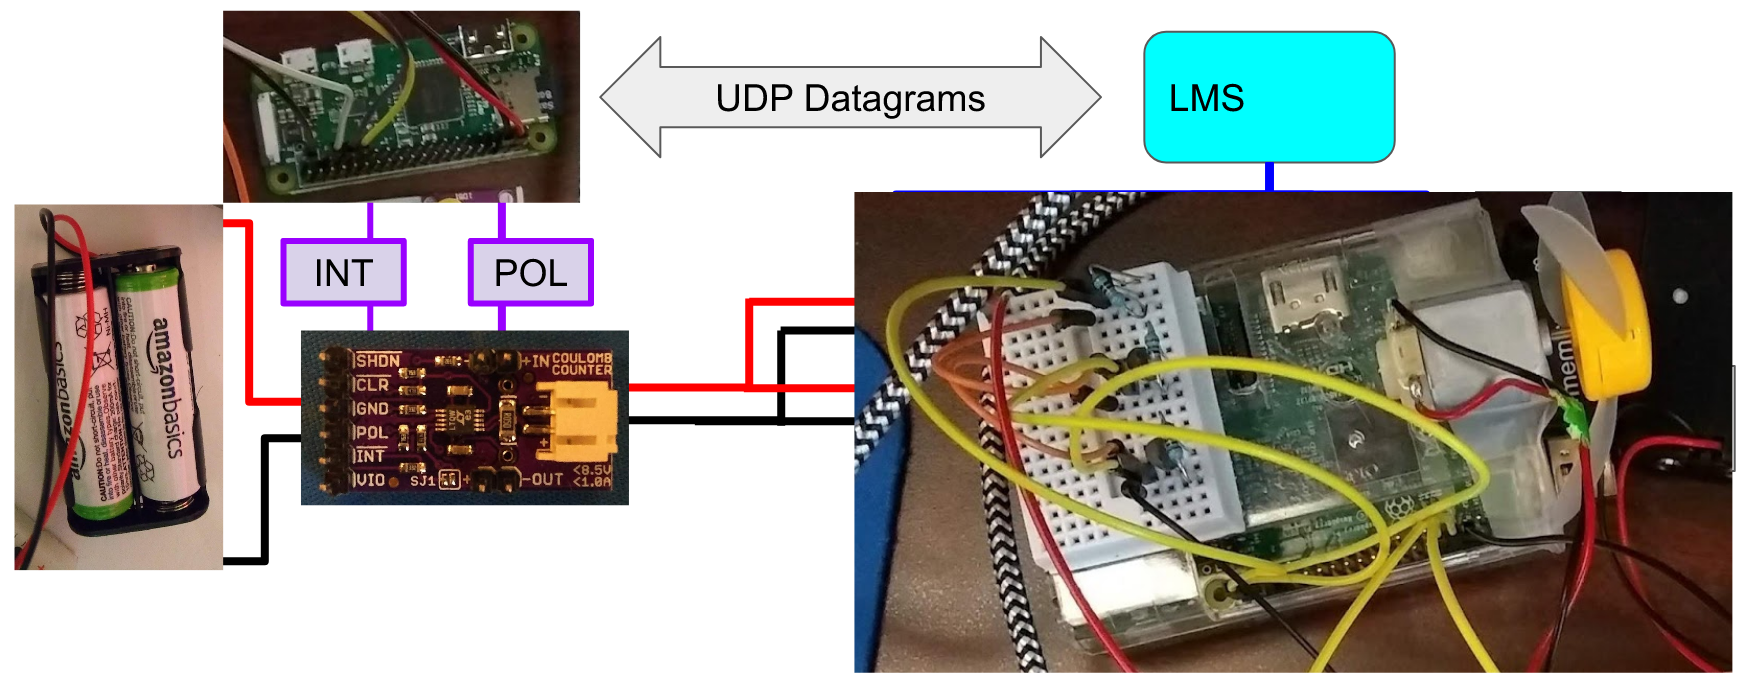
\includegraphics[width=6.5in]{img/uBmsModelPics.png}
    \caption{BMS and LMS Schematic}
    \label{fig:bmsModelPics}
\end{figure}

\subsection{System Model Cost}
The total cost for all materials is under 100 USD with item-specific prices list below:
\begin{itemize}
    \item Raspberry Pi 3            - 40 USD
    \item Basic Electronics Kit     - 30 USD
    \item LTC4150 Module            - 12 USD
    \item AA Battery case           -  8 USD
    \item Raspberry Pi Zero W       -  5 USD
\end{itemize}

\section{Request-Based Communication Protocol}\label{sec:rbComm}
Using the hardware presented in the previous section, the BMS and LMS are now capable of describing their respective supplies and demands via the UDP connection.
To facilitate online anomaly detection, the following section describes the protocol used when the LMS intends to activate a load and draw power from the batteries.
The BMS uses this protocol to determine whether supplying electricity for the load is feasible and approves or denies the load as needed.

\subsection{Load Requests}
In practice, components and/or electronic subsystems have a voltage range that can be accepted as input.
Such systems are also bounded in the amount of current they may draw.
This information can be used to model any load in control by the LMS.

Each load in control of the LMS is modeled using the four basic parameters described above: min/max voltage and min/max current.
Together, voltage and current give a min/max power draw for the particular load.
Each load is then transformed into a load request when the following parameters are also specified: release time, duration, deadline, and a unique token.
Release time specifies when the load may become active, duration specifies the maximum time for which the load will be active, and deadline specifies the time by which the load will no longer be active.
Although release time and deadline translate directly to real-time systems, duration may be thought of as worst-case execution time.
The unique token is used as a reference by the BMS and LMS when communicating so the full load request must only be transmitted once and then referred to by the unique token thereafter.

An example load request, constructed as a list of arguments in Python, may look like this:
\begin{lstlisting}
(0,         #Min voltage    (Volts)     (V)
 6,         #Max voltage    (Volts)     (V)
 0,         #Min current    (Amps)      (A)
 0.200,     #Max current    (Amps)      (A)
 0,         #Min Power      (Watts)     (W)
 1.2,       #Max Power      (Watts)     (W)
 10,        #Release time   (seconds)   (s)
 10,        #Duration       (seconds)   (s)
 0,         #Min Energy     (Joules)    (J)
 12,        #Max Energy     (Joules)    (J)
 120,       #Deadline       (seconds)   (s)
 0x0217)    #Unique Token   (hexadecimal)
\end{lstlisting}
which specifies a load with a voltage range of 0-6 volts (V), current range of 0-200 milliamp hours (mAh), power range of 0-1.2 Watts (W), release time of 10 seconds, duration of 10 seconds, energy range of 0-12 Joules (J), a deadline of 120 seconds, and a hexadecimal token 0x0217.

The load request template can be found on in the ubmsLoad.py file.

The LMS maintains a dictionary of load requests sent to the BMS which is updated whenever the BMS changes the accepted/rejected status of the request. 

\subsection{Load Request Replies}
Upon receiving a load request from the LMS, the BMS performs several comparisons.
The voltage range of the load is used to determine whether under- or over-voltage constraints apply.
For example, suppose the battery managed by the BMS were reconfigurable as a 12V or 24V battery. One load may require 24V supply while a second load may require a 12V supply. The BMS must either accept both loads at different time ranges (so it may reconfigure cells in between) or reject one of the loads.
Supplying 12V to the 24V-only system (or vice-versa) may cause undervoltage (or overvoltage) and damage components.

Similarly, current ranges may be used to determine whether the current battery configuration can support the minimum and maximum current draw expected from the load.
The maximum current draw may be compared against the maximum current output from the present cell configuration.
The minimum current draw will be used later to determine mismatched loads.

The power ranges are used to determine whether the battery configuration can sustain the peak power draw of a combined set of loads.

The energy ranges, like minimum current draw, are used later in anomaly detection.

Finally, the timing constraints are used to calculate the power and energy ranges from the baseline voltage and current ranges.
The timing constraints also allow the BMS to schedule loads which might otherwise be incompatible due to peak power draw.

After determining if the load request can be satisfied, the BMS replies using only the load requests unique token and an error code (if any such error code exists).
No error code (or an error code of 0) indicates the load request is accepted and is scheduled as defined.

\section{Anomaly Detection Methods}\label{sec:anomalyDetection}
Having established the structure of request-based communication between the BMS and LMS, the following section describes the anomaly detection methods used by the implementation.

\subsection{BMS Anomalies}
BMSs are responsible for monitoring a number of characteristics. These characteristics include, but are not limited to:
\begin{enumerate}
    \item State of Charge (SoC),
    \item Depth of Discharge (DoD),
    \item configuration,
    \item min/max voltage,
    \item min/max current,
    \item temperature,
    \item number of cycles,
    \item total power delivered,
    \item Open-Circuit Voltage (OCV),
    \item relaxation time, and
    \item communications
\end{enumerate}

It is possible for any combination of these parameters to deviate from expectations.
For the purpose of this work, we used the BMS modeling of the battery and the LMS modeling of loads (and thus load requests) to establish expectations.
Online anomaly detection, is possible based on the combination of the BMS battery model and LMS load requests.

\subsection{Anomalies Covered}
In this work, the proposed system model addresses five types of anomalies: over/under voltage, over/under current, and load mismatch.

\subsubsection{Over Voltage}
Overvoltage occurs when the voltage supplied by the battery exceeds the acceptable maximum input voltage of the load.
For example, using a 12V battery (ex. from an automobile) to directly power a 5V system (ex. a Raspberry Pi) may result in higher current and damage to the powered system.
Any load request whose minimum voltage range exceeds the battery's maximum configurable voltage range is rejected on the basis of overvoltage protection.

\subsubsection{Under Voltage}
Undervoltage occurs when the voltage supplied to a load falls below the acceptable minimum input voltage of the load.
For example, using a ~5V battery system (ex. the one in this model) to directly power an automobile starter motor (typically powered by a 12V lead acid battery), will likely prevent the load from performing properly.
In the worst case, undervoltage may lead to damage if unprotected field-effect transistors are used.

\subsubsection{Over Current}
Overcurrent occurs when the minimum current required by a load exceeds the maximum current for which the load is rated.
For example, suppose a phone charger is rated to draw at most 2.1A while charging.
If the charger were to begin drawing 5.0A, one might suspect a fault in the charger or overvoltage at the supply.
In either case, the result is out of the load specification and may be treated as a short-circuit.

\subsubsection{Under Current}
Undercurrent occurs when the current drawn by a load falls below the minimum current the load is expected to draw.
While this is not inherently dangerous, it may indicate an alternate load has been powered or that the powered load is malfunctioning.

\subsubsection{Load Mismatch}
A load mismatch occurs when the energy expended by the load exceeds the maximum energy range provided in the load request.
A load expending more energy than allotted indicates that it has either drawn more current over the allowed duration or exceeded the duration it claimed to be active.

A load mismatch also occurs when the load is activated before its release time or after its deadline. 
Although the load my have an acceptable voltage range, draw an acceptable amount of current, and not exceed the energy limits, activating outside the release time and deadline may interfere with other loads or push the peak power draw above acceptable limits.


\section{Experiments}\label{sec:experiments}
The anomaly detection described above was implemented on the BMS as a method of accepting and rejecting loads.
Implementation details of the online anomaly detection may be found at in the isProblemToSupply() function of ubmsSupply.py and in the periodic() function of bmsDriver.py.  
The following section describes how the experiments are setup and executed.

\subsection{Experimental Setup}
The experimental setup consisted of recreating the setup in Figure \ref{fig:bmsModelPics} with three key differences:
\begin{enumerate}
    \item the grounds of both Raspberry Pis are tied together,
    \item the Raspberry Pis are powered by external power supplies (so the builtin power protection circuitry is used), and
    \item only the fan and 100 Ohm resistive loads are used
\end{enumerate}

In the LMS Driver file (lmsDriver.py), several load requests are constructed.
Some load requests are known to be impossible or dishonest in advance but are created to test the BMS.

Each load request represents one of the five anomalies detected by the BMS.
The following list describes each load request name and its purpose:
\begin{enumerate}
    \item vHiArgs - Requests a supply voltage that is too high for the BMS
    \item vLoArgs - Requests a supply voltage that is too low for the BMS
    \item iHiArgs - Requests a max current that is too high for the BMS
    \item fanLoadArgs - Requests an honest voltage and current range to support the fan
    \item resLoadArgs - Requests an honest voltage and current range to support the 100 ohm resistor
    \item badFanLoad1Args - Requests a dishonest current range (too high) to support the fan
    \item badFanLoad2Args - Requests a dishonest current range (too low) to support the fan
\end{enumerate}

The first three load requests demonstrate anomaly detection prior to accepting loads as the requested loads are out of range of the BMS.
The fanLoadArgs and resLoadArgs requests are honest depictions of the fan and resistor loads.
The final two fan load requests are accepted until they are executed at which point the BMS detects the load mismatch between the requested load and the load that is being executed.

\subsection{Experimental Execution}
To run the experiment, the BMS and LMS are connected as depicted in Figure \ref{fig:bmsModelPics} with the exceptions noted above.
After each device is powered on, SSH is used to access the BMS and run bmsDriver.py.
Subsequently, SSH is used to access the LMS and run lmsDriver.py

The LMS will send load requests over UDP and await acceptance or rejection by the BMS.
After all load requests are handled, the schedule defined by the load requests is executed.

Each load request serves as a separate experiment described below.

\subsubsection{Over / Under Voltage}
The over and under voltage protection is tested by the vHiArgs and vLoArgs load request.
It is expected that these load requests should be rejected on the basis of their voltage range being outside the supplied voltage range of the battery and thus the BMS. 

\subsubsection{Over Current}
The overcurrent protection is tested by the iHiArgs load request.
It is expected that this load request should be rejected on the basis that its maximum current draw exceeds the allowable current draw from the battery.

\subsubsection{Under Current}
Since the NiMH battery does not have a minimum required current draw, undercurrent protection is tested by the badFanLoad1Args load request where the requested load exceeds the fan current draw.
It is expected that the load request should be accepted initially but rejected during the execution of this load (since the current draw is too low).

\subsubsection{Load Mismatch}
The badFanLoad2Args load request falsely claims the current draw of the fan is lower than it is.
This final load request demonstrates the detection of a load mismatch online where the fan current draw greatly exceeds the load request and thus the load should be rejected.

\section{Results}\label{sec:results}
The results of each experiment are displayed to the user through the BMS and LMS SSH terminals.
The following section presents the results of each load request and its subsequent rejection.

\subsubsection{Over / Under Voltage}
The first two loads (vHiArgs and vLoArgs) are rejected by the BMS on the basis of voltage being out of range.
Figure \ref{fig:vOutOfRange} shows the terminal output of the BMS indicating this error.
The LMS also receives a reply indicating these loads have been rejected as seen in Figure \ref{fig:lmsRejected}.
The unique tokens for the under and over voltage loads are 0xded1 and 0xded2.

\begin{figure}[!htbp]
    \centering
    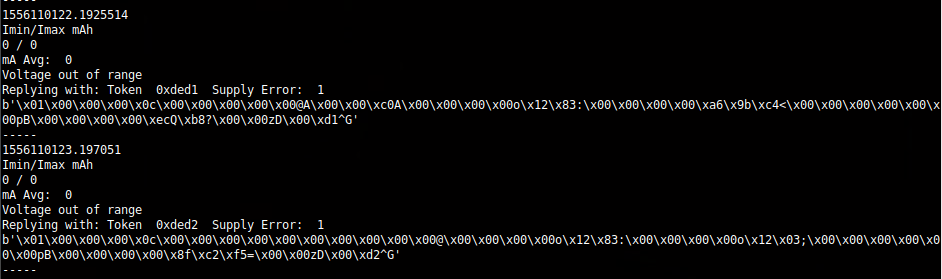
\includegraphics[width=6.5in]{img/vOutOfRange.png}
    \caption{BMS rejecting over/under voltage load requests}
    \label{fig:vOutOfRange}
\end{figure}
\begin{figure}[!htbp]
    \centering
    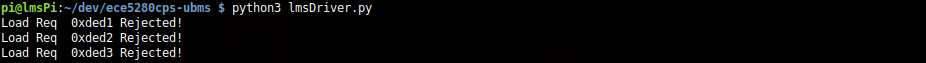
\includegraphics[width=6.5in]{img/lmsRejected.png}
    \caption{LMS receiving rejected load request replies}
    \label{fig:lmsRejected}
\end{figure}

\subsubsection{Over Current}
The third load (iHiArgs) is rejected by the BMS on the basis of the battery being unable to support the current range requested by the load.
Figure \ref{fig:iOutOfRange} shows the terminal output of the BMS indicating this error.
Figure \ref{fig:lmsRejected} also shows this third rejection with token 0xded3.

\begin{figure}[!htbp]
    \centering
    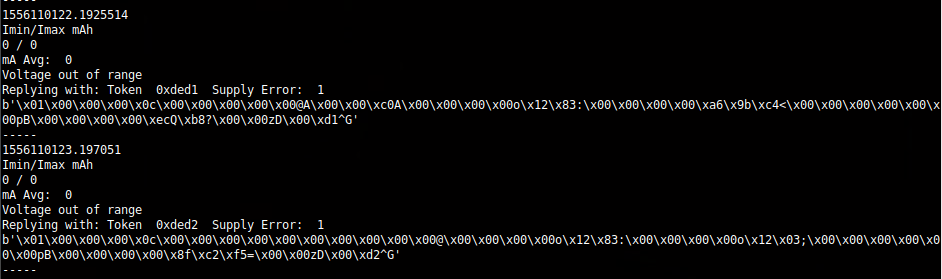
\includegraphics[width=6.5in]{img/vOutOfRange.png}
    \caption{BMS rejecting overcurrent load requests}
    \label{fig:iOutOfRange}
\end{figure}

\subsubsection{Under Current}
The undercurrent load (badFanLoad1Args) is also rejected by the BMS on the basis of the current draw being lower than the expected current draw.
Figure \ref{fig:iUnder} shows the terminal output of the BMS indicating this error.
The BMS also identifies which load is responsible for the undercurrent.
The LMS terminal also indicates the fan load is the only active load at the time in Figure \ref{fig:badFan1Active}.

\begin{figure}[!htbp]
    \centering
    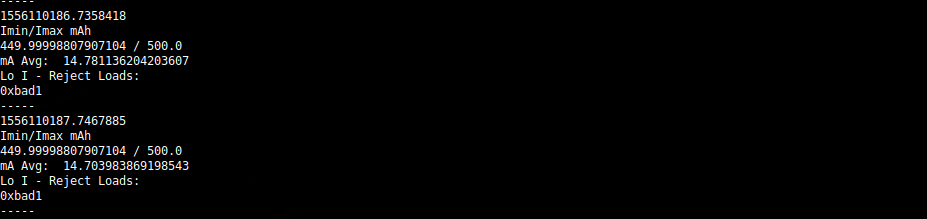
\includegraphics[width=6.5in]{img/iUnder.png}
    \caption{BMS rejecting undercurrent load requests}
    \label{fig:iUnder}
\end{figure}
\begin{figure}[!htbp]
    \centering
    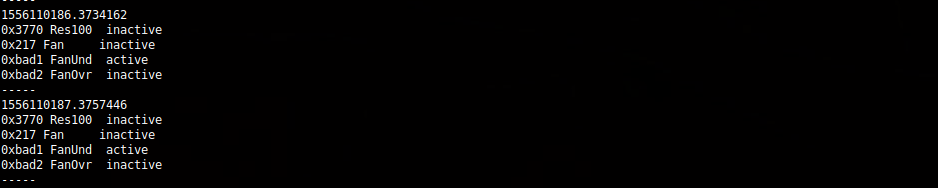
\includegraphics[width=6.5in]{img/badFan1Active.png}
    \caption{LMS fanUnder (badFanLoad1Args) load active}
    \label{fig:badFan1Active}
\end{figure}

\subsubsection{Load Mismatch}
Finally, the mismatched load (badFanLoad2Args) is also rejected by the BMS as the current draw of the motor is much higher than the load request indicated.
Figure \ref{fig:iOver} shows the terminal output of the BMS indicating this error.
The LMS terminal also indicates the fan load is the only active load at the time in Figure \ref{fig:badFan2Active}.

\begin{figure}[!htbp]
    \centering
    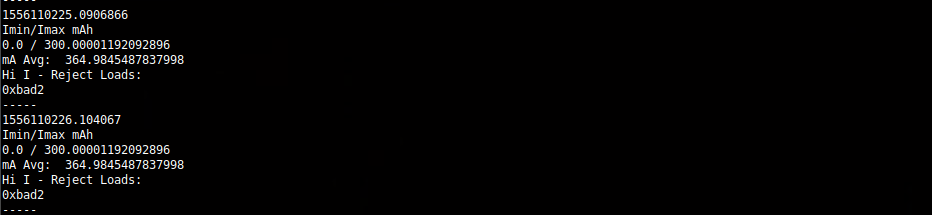
\includegraphics[width=6.5in]{img/iOver.png}
    \caption{BMS rejecting a load mismatch}
    \label{fig:iOver}
\end{figure}
\begin{figure}[!htbp]
    \centering
    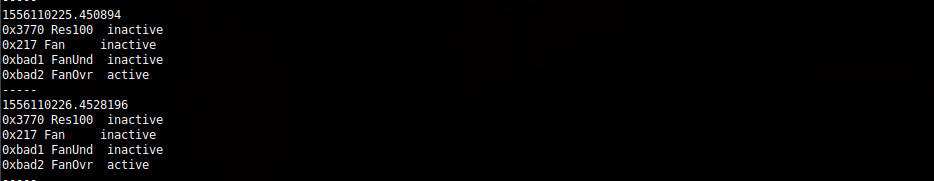
\includegraphics[width=6.5in]{img/badFan2Active.png}
    \caption{LMS fanOvr (badFanLoad2Args) load active}
    \label{fig:badFan2Active}
\end{figure}

\section{Discussion}\label{sec:discussion}
The following section discusses some model weaknesses, implementation challenges, deferred objectives, and course-related work.

\subsection{Model Weaknesses}
During the development of this project, several weaknesses became apparent.
The following subsections describe these weaknesses.

\subsubsection{Coulomb Counters as a Restriction}
A coulomb counter was chosen as the measurement device with the (mis)understanding that it could dually serve as a method of monitoring current flow.
After installing the hardware and creating an ISR to service the interrupts, it became apparent that smaller current draws correlated to less frequently firing interrupts.
However, there was no means by which the coulomb counter could be used to sample the instantaneous current.
Thus, while the coulomb counter served well as a "battery fuel gauge" it made current detection more difficult than intended.
Were this project to be repeated, a shunt would be used in conjunction with the coulomb counter to allow for instantaneous current sampling.
For context, a shunt is a small-valued resistor across which voltage may be sampled.
Ohm's law ($V=IR$) provides an explicit relationship between the voltage across the small-valued resistor and the current flowing through it.
With the appropriate hardware, the Raspberry Pi GPIO could sample the voltage across the shunt whenever a current measurement was necessary and use the coulomb counter only as a fuel gauge.

This oversight resulted in inappropriate current readings when loads shifted from high current to low current as the firing frequency of the coulomb counters ISR drops significantly when switching from the fan load to the resistor load.
The remedy (without using a shunt) was to use the time since the last sample to continually adjust the current estimate.
Still, the resultant calculation is only an estimate - a shortcoming of this approach.

\subsubsection{No Priorities or Conflict Resolution}
In the case where multiple loads are scheduled atop one another, no priority scheme is established to decide which loads should be rejected.
As an example, suppose an electric vehicle can power heated seats while also driving motors.
The driver wishes to drive 40 miles independent of whether the heated seats are enabled.
If the combination of driving and using heated seats requires more energy than the battery can supply, both will be rejected.

In practice, a better approach would be to reject the lower-priority load request or adjust the lower-priority load request to reduce power consumption.
A practical realization of this approach would be to run the heated seat as on a 50\% duty cycle rather than keep them active the entire time.

\subsubsection{Hidden Loads}
Another weakness is the possible of parasitic loads hiding in the "wake" of larger loads (and thus larger load requests).
For example, suppose a motor requests to draw 100A maximally.
If the motor only draws 80A of the 100A allotted, a parasitic (or malicious) load on the power bus could wait until the motor's load request was active to consume the difference in power between the motor's actual current draw and its allotted current draw.
Thus, 20A could be consumed by another system that did not file a load request without being detected.
Thus, while the practice of using request-based communication may mitigate some anomalies it also opens up an attack surface.

\subsection{Implementation Challenges}
As mentioned in the discussion of coulomb counters above, development of the BMS and LMS led to the discovery of several challenges when realizing the system.
The following section describes some challenges encountered.

\subsubsection{Hardware}
The greatest difficulties in implementation came from misunderstanding the Controller Area Network (CAN) implementation requirements.
The original intent was to use a CAN bus to communicate between the BMS and LMS as would likely be done in an automotive setting.
However, the microcontrollers originally used (PIC18Fs) were not equipped to be used with the CAN transceivers originally purchased.
The CAN controller required for communicating with the transceivers was missing and could not be replicated with the hardware on hand.
Thus, communication was performed through wireless interfaces on the Raspberry Pis.

\subsubsection{Software}
The only "problem" encountered in software development was an issue of packaging class variables when sending the variables over UDP.
It was expected that Python would list all class variables consistently when calling the vars(), local(), and global() functions.
Interestingly, despite enumerating variables in a fixed order (as seen by the load request example) there is no guarantee the variables will be listed in the order they are initialized.

This problem, although simple in hindsight, consumed a fair amount of time when debugging UDP communications.
The lesson, as always, is to never assume anything about the software implementation that lies beneath.

\subsection{Deferred Objectives}
As mentioned in the implementation challenges above, the switch from CAN to wireless interfaces occurred after a misunderstanding about CAN transceivers.
The following section discusses objectives deferred due to time, hardware, software, or other issues.

\subsubsection{Controller Area Network Communication}
As mentioned above, a CAN bus was originally intended to carry the communication of load requests and replies between the BMS and LMS.
This objective was deferred as the incorrect hardware was purchased and the necessary hardware would not arrive in time to finish the project.
As such, wireless communication and UDP was used in place of the CAN bus.

\subsubsection{Min/Max Energy Consumption}
The original intent of establishing energy ranges was to hold loads accountable for drawing too much or too little energy.
Due to time constraints, this feature was not implemented.

\subsubsection{Peak Shaving via Sliding Windows}
Although the "duration" term in load requests is provided primarily as a means of calculating expected energy usage, duration also gives the BMS the freedom to power the load anywhere in the time window between "release time" and "deadline".
In real-time systems, the scheduler is responsible for allocating WCETs such that all jobs are completed before their deadline and no WCETs overlap.
In a BMS, however, it is acceptable for loads to overlap - in fact, it is a requirement for most BMSs.
However, when scheduling loads it is important that the peak power draw not exceed the peak power output of the battery.
Beyond this, however, it is beneficial for the BMS to minimize the peak power draw even if the set of loads scheduled is already feasible.
Lowering the peak power draw extends battery life and wastes less energy via Joule Heating.

The project was originally intended to provide some form of peak shaving by treating load requests as a type of demand that could "slide" within the window of "release time" and "deadline".
Due to time constraints, this objective was deferred.

\subsection{Course Related Work}
This project is part of the Wayne State University Department of Electrical and Computer Engineering's ECE 5280 Cyber-Physical Systems course.
The following section describes the sensors, actuators, and ISRs used in this project and how they relate to course material.

\subsubsection{Sensors}
The sensors used in this project include the coulomb counter, GPIO input pins, and system clock.
The coulomb counter is a standalone integrated circuit which interrupts the LMS each time a fixed value of electric charge passes through the coulomb counter.
In this manner, the coulomb counter acts as a current measurement device and a "battery fuel gauge".

The GPIO pins on the BMS act as input devices which sense changes in the voltage supplied by the coulomb counters interrupt (INT) and polarity (POL) pins.
The GPIO INT input is assigned to an ISR (described later) while the GPIO POL input is sampled as needed. 

The system clock (of both Raspberry Pis) is used as a means of synchronization when activating (by the LMS) and detecting (by the BMS) loads.
Although the system clock does not explicitly "sense" any change in the state of the hardware, it does determine the rate at which time passes and acts as the signaling mechanism for enabling and disabling loads.

\subsubsection{Actuators}
The actuators used in this project include the fan, GPIO pins, and transistors.
The fan, the largest system load, imparts force on the air around the system.
Although the airflow is not measured in any way by the system, actuation is still performed.

The GPIO pins on the LMS are used to activate loads based on the system clock and coulomb counter (accessed by the BMS).
These GPIO pins enable and disable the PN2222a transistors which allow current flow to the system loads.
The PN2222a transistors are the only actuators whose output and change imparted on the system is measured.
Since the PN2222a transistors control current flow from the battery to loads, the coulomb counter is used to determine whether the transistors are functioning appropriately.

\subsubsection{Interrupt Service Routines}
As mentioned above, the coulomb counter fires an interrupt (INT) each time a fixed value of charge passes through the counter.
The BMS, therefore, has an ISR defined in the BMS driver (bmsDriver.py) responsible for handling the interrupt.
The ISR is also responsible for sampling the polarity (POL) pin of the coulomb counter to determine direction.

\section{Conclusion and Future Work}\label{sec:conclusion}
In conclusion, this work provides a low-cost implementation of a BMS and LMS with online anomaly detection.
Request-based communication over UDP is used as the basis for anomaly detection by the BMS and the LMS provides activation and deactivation of loads according to the BMS acceptance or rejection of lead requests.

Future work for this project include addressing the deferred objectives described in Section \ref{sec:discussion}, Discussion, and extending the load characteristics that may be used when detecting anomalies including, but not limited to:
\begin{enumerate}
    \item power-on profile,
    \item duty cycle, and
    \item load-request adjustment by the BMS
\end{enumerate}

As previously mentioned, all digital resources (including this report) can be found on:\\
https://github.com/aarontwillcock/ece5280cps-ubms

\bibliography{uBms}
\bibliographystyle{abbrv}

\end{document}
